\documentclass[11pt,a4paper,titlepage]{report} 
\usepackage[utf8]{inputenc} 
\usepackage[french]{babel} 
\usepackage[T1]{fontenc} 
\usepackage{amsmath} 
\usepackage{amsfonts} 
\usepackage{amssymb} 
\usepackage{hyperref}
\usepackage{graphicx} 
\usepackage{verbatim}
\usepackage[final]{pdfpages} 
\usepackage[toc,page]{appendix} 
\usepackage[top=2.5cm,bottom=2.5cm,right=2.5cm,left=2.5cm]{geometry} 

\newcommand{\HRule}{\rule{\linewidth}{0.5mm}}

\begin{document}
\renewcommand{\thefootnote}{\fnsymbol{footnote}}
\begin{titlepage}
\begin{center}

% Upper part of the page. The '~' is needed because \\
% only works if a paragraph has started.
%
\includegraphics[width=0.15\textwidth]{./logo}~\\[1cm]

\includegraphics[width=0.15\textwidth]{logo.png}~
\\[1cm]
\textsc{\LARGE iut informatique de belfort-montbéliard}\\[1cm]

\textsc{\Large Projet de base de données}\\[0.5cm]

% Title
\HRule \\[0.4cm]
{ \huge \bfseries Velacampus website \\[0.4cm] }

\HRule \\[1.5cm]

% Author and supervisor
\begin{minipage}{0.4\textwidth}
\begin{flushleft} \large
\emph{Auteur:}\\
Morgane \textsc{cabrol}\\
Pierre \textsc{limballe}\\
Geoffrey \textsc{glangine}\\
Auguste \textsc{meyer}
\end{flushleft}
\end{minipage}
\begin{minipage}{0.4\textwidth}
\begin{flushright} \large
\emph{Superviseur:} \\
Alexandru  \textsc{dobrila}
\end{flushright}
\end{minipage}
\\[1cm]
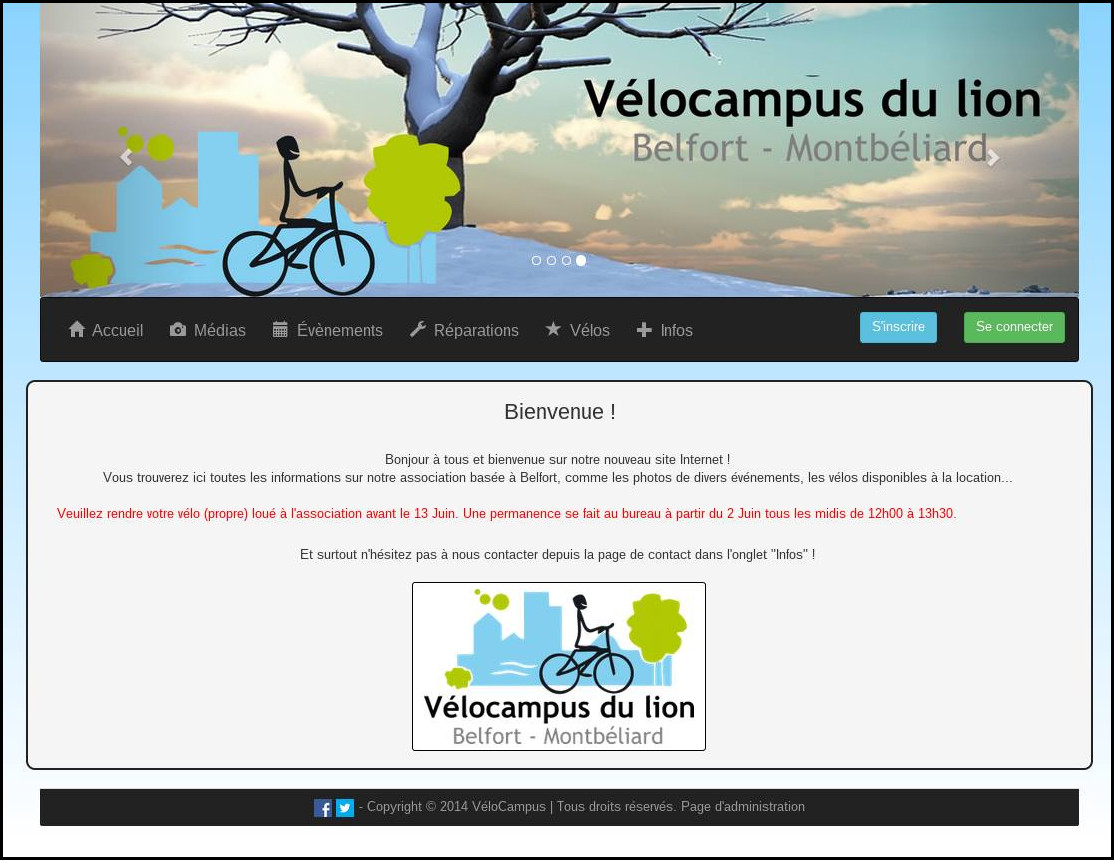
\includegraphics[width=0.8\textwidth]{site.jpg}~
\\[1cm]
\vfill

% Bottom of the page
{\large \today}

\end{center}
\end{titlepage}

\tableofcontents
\chapter*{Introduction}
Vélocampus est une association louant des vélos aux étudiants à très petit tarifs. De plus, elle s’occupe de la réparation et de l'entretien de vélos loués ou non.

Pour ce projet, nous avons voulu réaliser un site permettant à Vélocampus de gérer son administration plus facilement. Pour cela nous vous présenterons d'abord le cahier des charges que nous avons conçus avec les membres de l'association, puis nous expliquerons la base de données que nous avons décidés de mettre en place, ainsi que les fonctionnalités que nous avons implémenté sur le site. Enfin, nous aborderons les problèmes que nous avons rencontrés puis, les améliorations qui pourraient être apporté au site par la suite.


\chapter{Le cahier des charges}
Après une réunion avec les membres de l'association, nous sommes arrivés à la conclusion que le site contiendrait une petite partie client, rendant ainsi l'association présente sur le web et une grosse partie administration, permettant toutes la gestions de l'association. 
Nous avons finalement construit ce cahier des charges :\\


\section{La partie administration :} 
Elle sera accessible à tous les membres de l'association \\
\begin{itemize}
\item Une mailing liste des adhérents \\
\textit{(Permettant à l'administrateur d'importer la liste sur une boite mail afin de pouvoir envoyer des messages groupés)}
\item Un Suivi des vélos \\
\textit{(Afin de savoir quel vélo est en location, quel vélo a subit quel réparation...)}
\item Une gestion des demandes d'adhésions faites en lignes 
\item Une messagerie internet \\
\textit{(Permettant aux différents administrateurs de communiquer entre eux)}
\item Une gestion des vélos \\
\textit{(Pour ajouter des vélos, supprimmer des vélos ou encore modifoer des vélos)}
\item Une gestion de réparation \\
\textit{(Permettant d'ajouter des réparations à certain vélo et de connaitre le prix de ces réparations)}
\item Une gestion du site publique \\
\textit{(Ajouter des photos, modifier les partenaires, modifier le messages d'acceuil ...)}
\item L'importation d'un calendrier Gmail \\
\textit{(Permettant d'importer un calendrier d'évenement sur la partie client du site et d'afficher le calendrier interne de l'association sur la partie administration du site)}
\end{itemize}

  
  
\section{ La partie client :}

\begin{itemize}
\item Une formulaire d'adhésion \\
\textit{(Permettant aux visiteurs de s'inscrire en ligne)}
\item Un formulaire de demande de réparation \footnote{Cette partie n'est accessible que par les adhérents connectés}  \\
\textit{(Permettant aux adhérents de demander la réparations de leurs vélos )}
\item Calendrier en ligne avec les événements de l'association 
\item Une page d'informations  \\
\textit{(Contenant la présentations de l'association, ses membres et ses partenaires)} 
\item Une page de photos et videos  

\end{itemize}
\chapter{Base de données}
\section{le modèle conceptuel de donnée}
\begin{center}
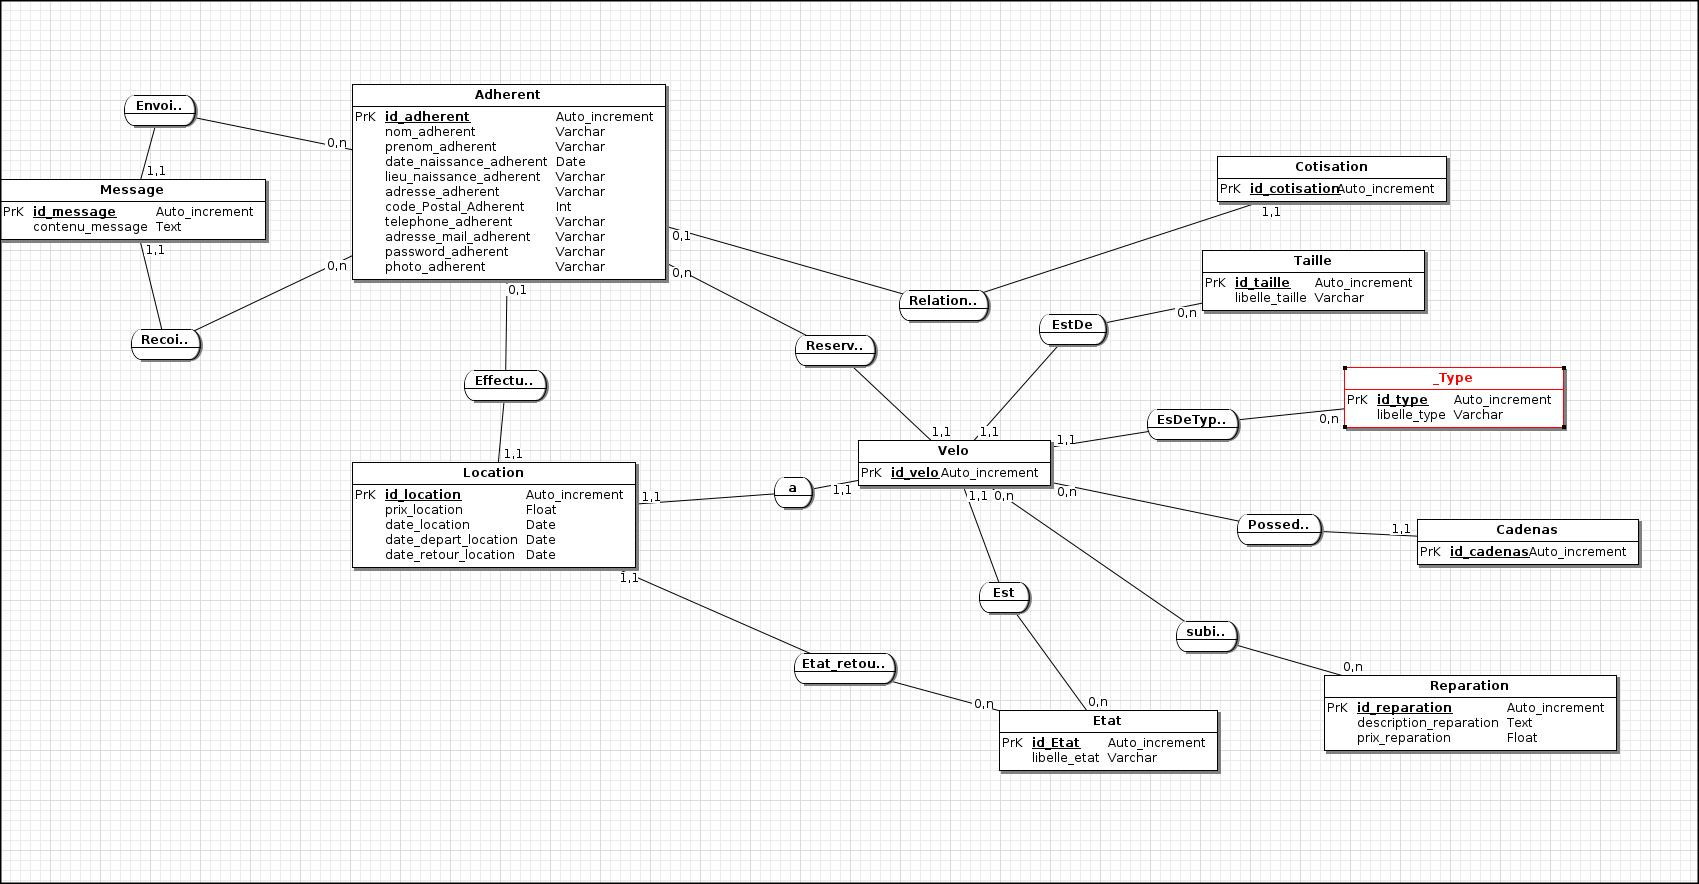
\includegraphics[width=1\textwidth]{MCD.jpg}~
\end{center}

\section{La réalisation du MCD}

\chapter{Le fonctionnement du site Internet}
Le site est organisés en deux parties, une partie administration assez conséquente et une partie client.
\section{La Structure}
Tous d'abord nous avons utilisés GITHUB qui est un très bonne outils de gestion de développement.
Vous pouvez trouvez notre projet à ce lien :
\url{https://github.com/kwidz/VeloCampus}
De plus nous avons utiliser un framework CSS : Bootstrap, pour que notre site internet s'adapte à tous type d'écrans sans trop de problèmes.
Enfin, afin de ne pas se perdre dans tous les fichiers, nous avons suivi une struture assez simple : Nous avons plusieurs fichiers :
\begin{itemize}
\item index.php \\
\textit{(Ce fichier inclue les différentes pages html)}
\item footer.html
\item header.html
\item menu.html \\
\textit{(Ce fichier contient le menu que l'utilisateur vois lorqu'il n'est pas connecté)}
\item menulog.html \\
\textit{(Ce fichier contient le menu que l'utilisateur vois lorqu'il est connecté)}
\end{itemize}
 puis des dossiers portant le noms de chaques sous partie du menu, contenant un dossier de traitement ainsi qu'un index.
 
\section{Les fonctions importantes}
Ce projet comporte beaucoup de fonctionnalités donc pour la suite nous expliquerons le fonctionnement que de certaines parties.  
\subsection{La partie location}
La partie Location se trouve dans la partie admistration, elle permet de : 
\begin{itemize}
\item Créer une location
\item Voir les vélos non loués
\item Voir les personnes qui n'ont pas encore rendu leurs vélos
\item Voir toutes les locations de l'année
\item Ajouter un retour de location 
\end{itemize}

Cette partie a été délicate à gérer car lorsque l'on loue un vélo il faut connaître son état, la date de location, les noms des cadenas qui sont loués avec le vélo ainsi que les informations de l'adhérent qui loue le vélo. Il nous a donc fallut faire plusieurs jointure.\\

Par exemple : Cette requete sert à afficher les vélos non-loués. 
\begin{verbatim}
Select v.id_velo, c.id_cadenas, ty.libelle_type, t.libelle_taille from Velo v, Cadenas c, Taille t, _Type ty where v.id_velo not in(Select id_velo from Location where date_retour_location is null ) and c.id_velo=v.id_velo and v.id_type=ty.id_type and v.id_taille=t.id_taille order by(id_velo) 
\end{verbatim} 

De plus lorsque l'adhérent retourne son vélo, l'administrateur doit pouvoir modifier l'état du vélo et ajouter une date de retour. 

\subsection{L'affichage des demandes}
Lorqu'un fait une demande sur le site publique, celle ci est affiché sur la page administration en attente d'être validé ou refusé.

La demande d'inscription est validée si les informations données sont correcte et si la personne qui a fait cette demande est venu payer la cotisation à l'association. C'est seulement à ce moment que la personne pourra se connecter sur le site publique.

Voici un exemple :\\
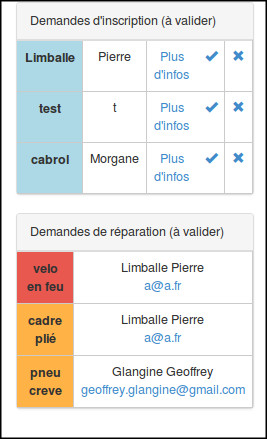
\includegraphics[width=0.5\textwidth]{demande.jpg}~

Si l'on clique sur le bouton valider à coter d'un prénom, la personne sera ajouté à la table cotisation qui contient toute les personnes cotisantes.
\begin{verbatim}
INSERT INTO Cotisation (`id_cotisation`, `id_adherent`) VALUES (NULL, ".$_GET['id'].");
\end{verbatim} 
Par contre si l'on clique sur le bouton supprimer, la personne sera enlévé de la table adhérent.
\begin{verbatim}
DELETE  from Adherent where id_adherent='".$_GET['id']."'
\end{verbatim}

\subsection{L'ajout d'image}
Nous voulions créer une fonctionnalité simple qui permettrait aux membres de Vélocampus d'ajouter ou supprimer des photos sur leur site. De plus nous ne voulions pas ajouter seulement un lien vers l'image dans la base de donnée car nous voulions que lors de la suppression d'image, l'image soit réellement supprimer et pas seulement le lien qui mène à elle dans la base de donnée.
\begin{center}
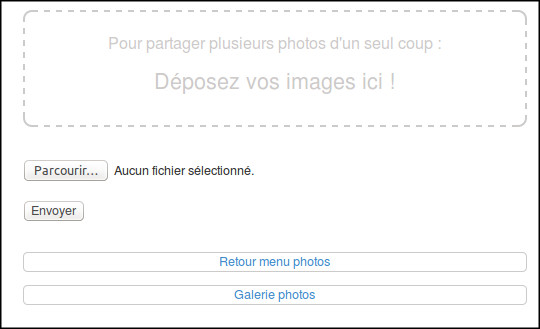
\includegraphics[width=0.3\textwidth]{addImage.jpg}~
\end{center}



\chapter{Les problèmes rencontrés}

\section{Adblock :} 
Adblock est une extension informatique permettant de bloquer les publicités sur les navigateurs. Elle est donc installé sur beaucoup d'ordinateur. 
Malheureusement, elle ne bloque pas que les publicités, lors de la réalisation du projet nous nous sommes aperçu que celle ci bloquait aussi toutes les actions ajax du site (qui nous permettaient le plus souvent de sécuriser le site) 
Nous avons donc du modifier notre façon de fonctionner. cela nous a fait perdre un peu de temps.

\section{La sécurité : }
Ce projet étant utilisés par la suite sur internet, il était primordiale de le sécuriser. Or, nous n'avons aucun cours sur la sécurité internet à l'IUT, nous avons donc du étudier cette aspect de l'informatique par nous même. Cela nous a donc apporté une charge de travail supplémentaire.

\section{Répartition du travail : }
Finalement, le plus gros problème que nous avons rencontrés est la répartition du travail. 
Le chef de projet a d'abord partagé les premières taches en pensant vérifier à la fin de la semaine leurs réalisations pour, ensuite, pouvoir en fournir d'autre. Malheureusement, seul trois membres ont travaillés, le quatrième n'avait absolument rien réalisé à la fin de la semaine. 
La tache de celui-ci étant indispensable pour la suite, le chef de projet a préféré la coder lui même car il s'est rendu compte qu'elle ne serait jamais faites.
Ce petit manège a recommencer à chaque nouvelle distribution de taches. C'est seulement à la fin du projet que l'élève en question a fini par avouer qu'il avait décidé de ne rien faire pour ce projet car la matière n'était pas assez importante à ses yeux. Cette mésaventure nous a fait perdre beaucoup de temps car nous avons souvent du attendre sur le travail de l'élève en question pour continuer à avancer. De plus, nous avons du travailler plus pour rattraper le travail manquant de se membre.
Ce projet étant difficilement réalisable à quatre, la difficulté a évolué dès lors que nous sommes passé à seulement trois membres actifs. 
\chapter{Les améliorations possibles}
Ce projet n'étant pas entièrement réalisable en un mois, ils restent beaucoup de fonctionnalités qui aurait put être implémenter plus tard, tels que : \\
\begin{itemize}
\item La réparation des vélos non loués 
\item La Demande de location en ligne \\
\textit{(Nous avons décider de ne pas la faire car il faut de toute façon se rendre à l'association pour récupérer le vélo loué.)}
\item Gestion des compte rendu de réunions \\ \textit{(Il faudrait créer un éditeur sur la partie administration du site afin que le secrétaire de l'association puisse noter directement en ligne le compte rendu des réunions et les sauvegarder en ligne.)} 
\item Ajout d'un forum \\
\textit{(L'association Vélocampus aurait aimé que nous mettions en place un forum pour tous les adhérents, nous avons malheureusement pas eu le temps)} 
\item Ajout d'une fontionnalité de paiement en ligne \\
\textit{(Nous aurions pu ajouter un lien paypal mais cela compliquait les choses plus qu'autres choses, de plus l'association préfère le contact humain.)} 
\end{itemize}
\chapter*{Conclusion}
\end{document}



